%
% domain.tex -- Definitionsbereich der DGL 40000019
%
% (c) 2018 Prof Dr Andreas Müller
%
\documentclass[tikz]{standalone}
\usepackage{amsmath}
\usepackage{times}
\usepackage{txfonts}
\usepackage[utf8]{inputenc}
\usepackage{graphics}
\usepackage{ifthen}
\usepackage{color}
\usetikzlibrary{arrows,intersections}

\begin{document}
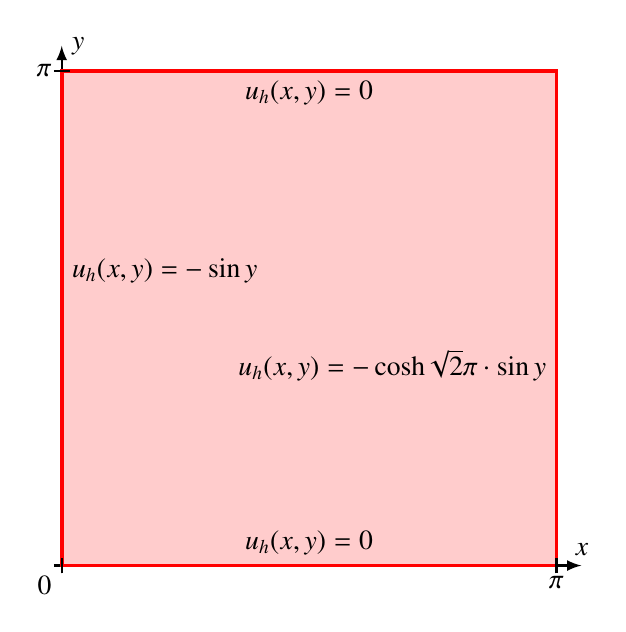
\begin{tikzpicture}[>=latex,thick]
\fill[color=red!20] (0,0) rectangle ({2*3.1415},{2*3.1415});
\draw[->] (-0.1,0)--(6.6,0) coordinate[label={$x$}];
\draw[->] (0,-0.1)--(0,6.6) coordinate[label={right:$y$}];
\draw[color=red,line width=1.4pt] (0,0)--({2*3.1415},0)--({2*3.1415},{2*3.1415})--(0,{2*3.1415})--cycle;
\draw (0,-0.1)--(0,0.1);
\draw ({2*3.1415},-0.1)--({2*3.1415},0.1);
\draw (-0.1,{2*3.1415})--(0.1,{2*3.1415});
\node at (0,{2*3.1415}) [left] {$\pi$};
\node at ({2*3.1415},0) [below] {$\pi$};
\node at (0,0) [below left] {$0$};

\node at (3.1415,0) [above] {$u_h(x,y)=0$};
\node at (3.1415,{2*3.1415}) [below] {$u_h(x,y)=0$};
\node at (0,{3.1415+0.6}) [right] {$u_h(x,y)=-\sin y$};
\node at ({2*3.1415},{3.1415-0.6}) [left] {$u_h(x,y)=-\cosh\!\sqrt{2}\pi\cdot\sin y$};

\end{tikzpicture}
\end{document}
